\section{Unblinding results}

This search for a new dark boson is done blindly to ensure that no bias is introduced in the
course of the analysis.
The data is unblinded in stages to ensure that the selection is behaving as expected on real data.

Before any unblinding the selection is first checked using data selected which is
consistent with the decay \decay{\Bd}{\jpsi\Kstarz}.
The selection applied in the \sm analysis of \btokstrmumu, as described in
\Ref{LHCb-CONF-2015-002}, yields $320\,000$ candidate decays.
Using the selection from \Sect{sec:db:sel} and approximately $\sim290\,000$
\decay{\Bd}{\jpsi\Kstarz} candidates remain,
therefore only $\sim10\%$ fewer events in this selection, which is not surprising
considering this search is for a much rarer process than \decay{\Bd}{\Kstarz\mumu} in the \sm.

Selected \decay{\Bd}{\jpsi\Kstarz} events are also used to check that the selection was not biased
based on either the year, or the polarity of the \lhcb magnet, while the data was collected.
No bias is observed.


The unblinding procedure begins by checking the yield of the normalization channel
\btokstrmumu in the range $1.1<\qsq<6.0\gevgev$ and comparing it with the yield from the \sm
analysis.
The yield is taken from an unbinned fit to selected prompt \btokstrdb candidates using a mass model
of
%same fit model for the signal component as used in \Ref{LHCb-CONF-2015-002}, which is the sum of
two Gaussian functions sharing the same mean, and with a power-law tail on the low mass side.
A simple exponential models the background component.
This yields 525 \Bd candidates, which can be compared to \approx$625$ events in the \sm selection,
where the drop in signal is, again, expected given the search is for a rare process.
Together with the drop in signal, comes a drop in background yield, from \approx$630$ background
events over the full mass range, to only 290.
Figure~\ref{fig:db:norm} shows the \Bd candidate mass spectrum for the normalization channel, and
the fitted distribution overlayed.

\begin{figure}
  \begin{center}
    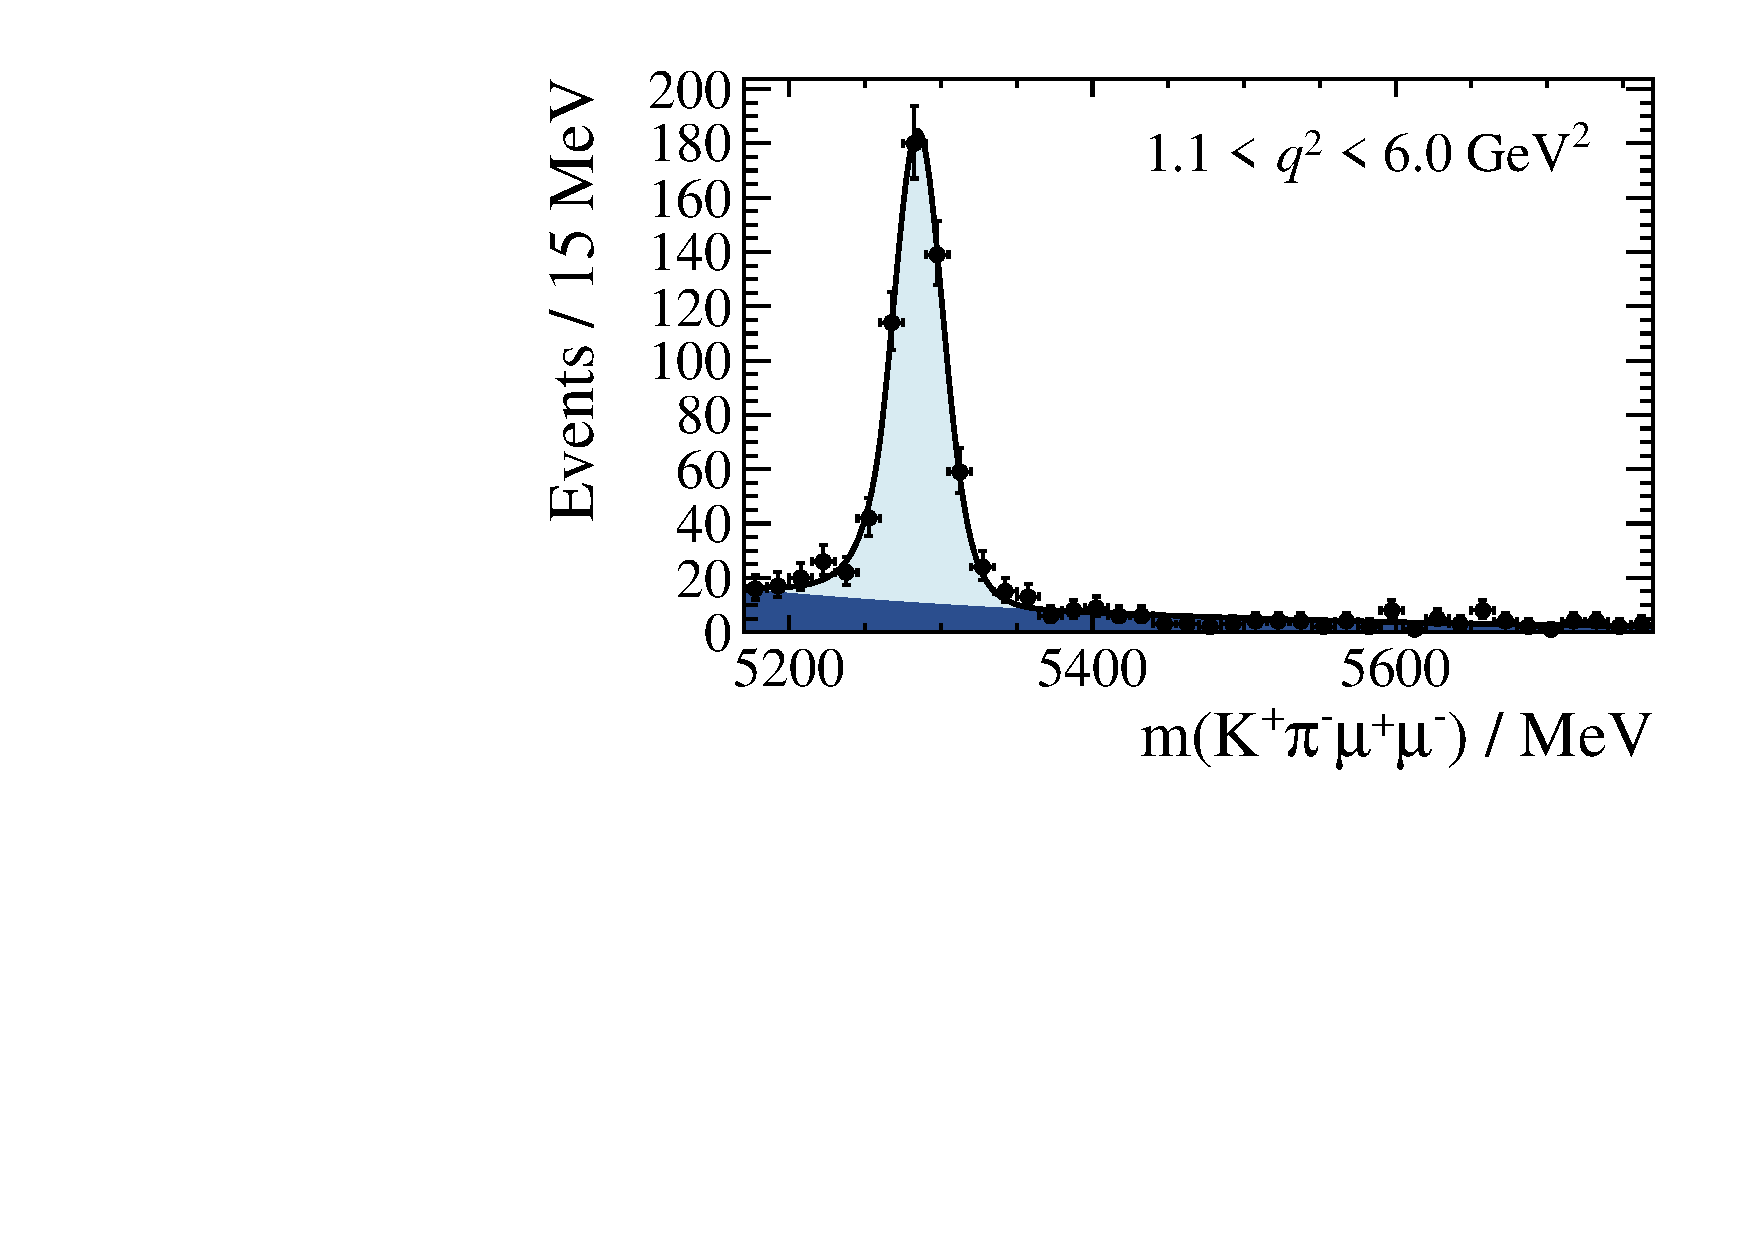
\includegraphics[width=0.48\textwidth]{norm_channel}
    \caption[Fit to the normalization channel, \btokstrmumu in the range $1.1<\qsq<6.0\gevgev$]
    {
      Fit to the invariant mass spectrum of the \Bd candidates in selected data in the range
      $1.1<\qsq<6.0\gevgev$.
      The signal model is the sum of two Gaussian functions with power-law tails on the low-mass
      side with parameters taken from the analysis described in
      Ref.~\protect\cite{LHCb-CONF-2015-002},the background model is a decaying exponential.
      This fit results in a signal yield of $(625\pm26)$ compared to approximately 625 in the \sm
      analysis.
      %for more in depth numbers, please refer to Table~\protect\ref{tab:db:nums126}.
    }
    \label{fig:db:norm}
  \end{center}
\end{figure}

After unblinding the region $1.1<\qsq<6.0\gevgev$, other prompt \qsq regions were also used to
confirm that the ratio of \bdt selection efficiencies
$\varepsilon_\mathrm{BDT}^\mathrm{\qsq bin} / \varepsilon_\mathrm{BDT}^{\decay{\Bd}{\jpsi\Kstarz}}$
are approximately the same in data and simulation.
To determine these efficiencies, the full selection without the \BDT is taken, and a fit performed
and the signal yield is extracted.
Next, the \BDT is applied and a second fit is performed, then take the ratio of the signal
yields.
A comparison between these numbers in data and simulation is shown in comparison is shown in
\Fig{fig:bdtEffRatio}, the two distributions are shown to be in good agreement, centred around
unity with about 5--10\pc precision.
%This approach ignores the fact that there may be some small peaking background component that gets
%counted as signal pre-BDT cut, but is removed by the BDT.
%Note, however, that in the
%$\varepsilon_\mathrm{BDT}^\mathrm{\qsq bin} / \varepsilon_\mathrm{BDT}^{\decay{\Bd}{\jpsi\Kstarz}}$
%ratio, only the difference in peaking background contributions matters.
%Given that all peaking backgrounds that are visible in the various 2-body mass combinations are
%explicitly vetoed, no peaking background contributions at the level of the statistical precision of
%this test are expected.

\begin{figure}
  \begin{center}
    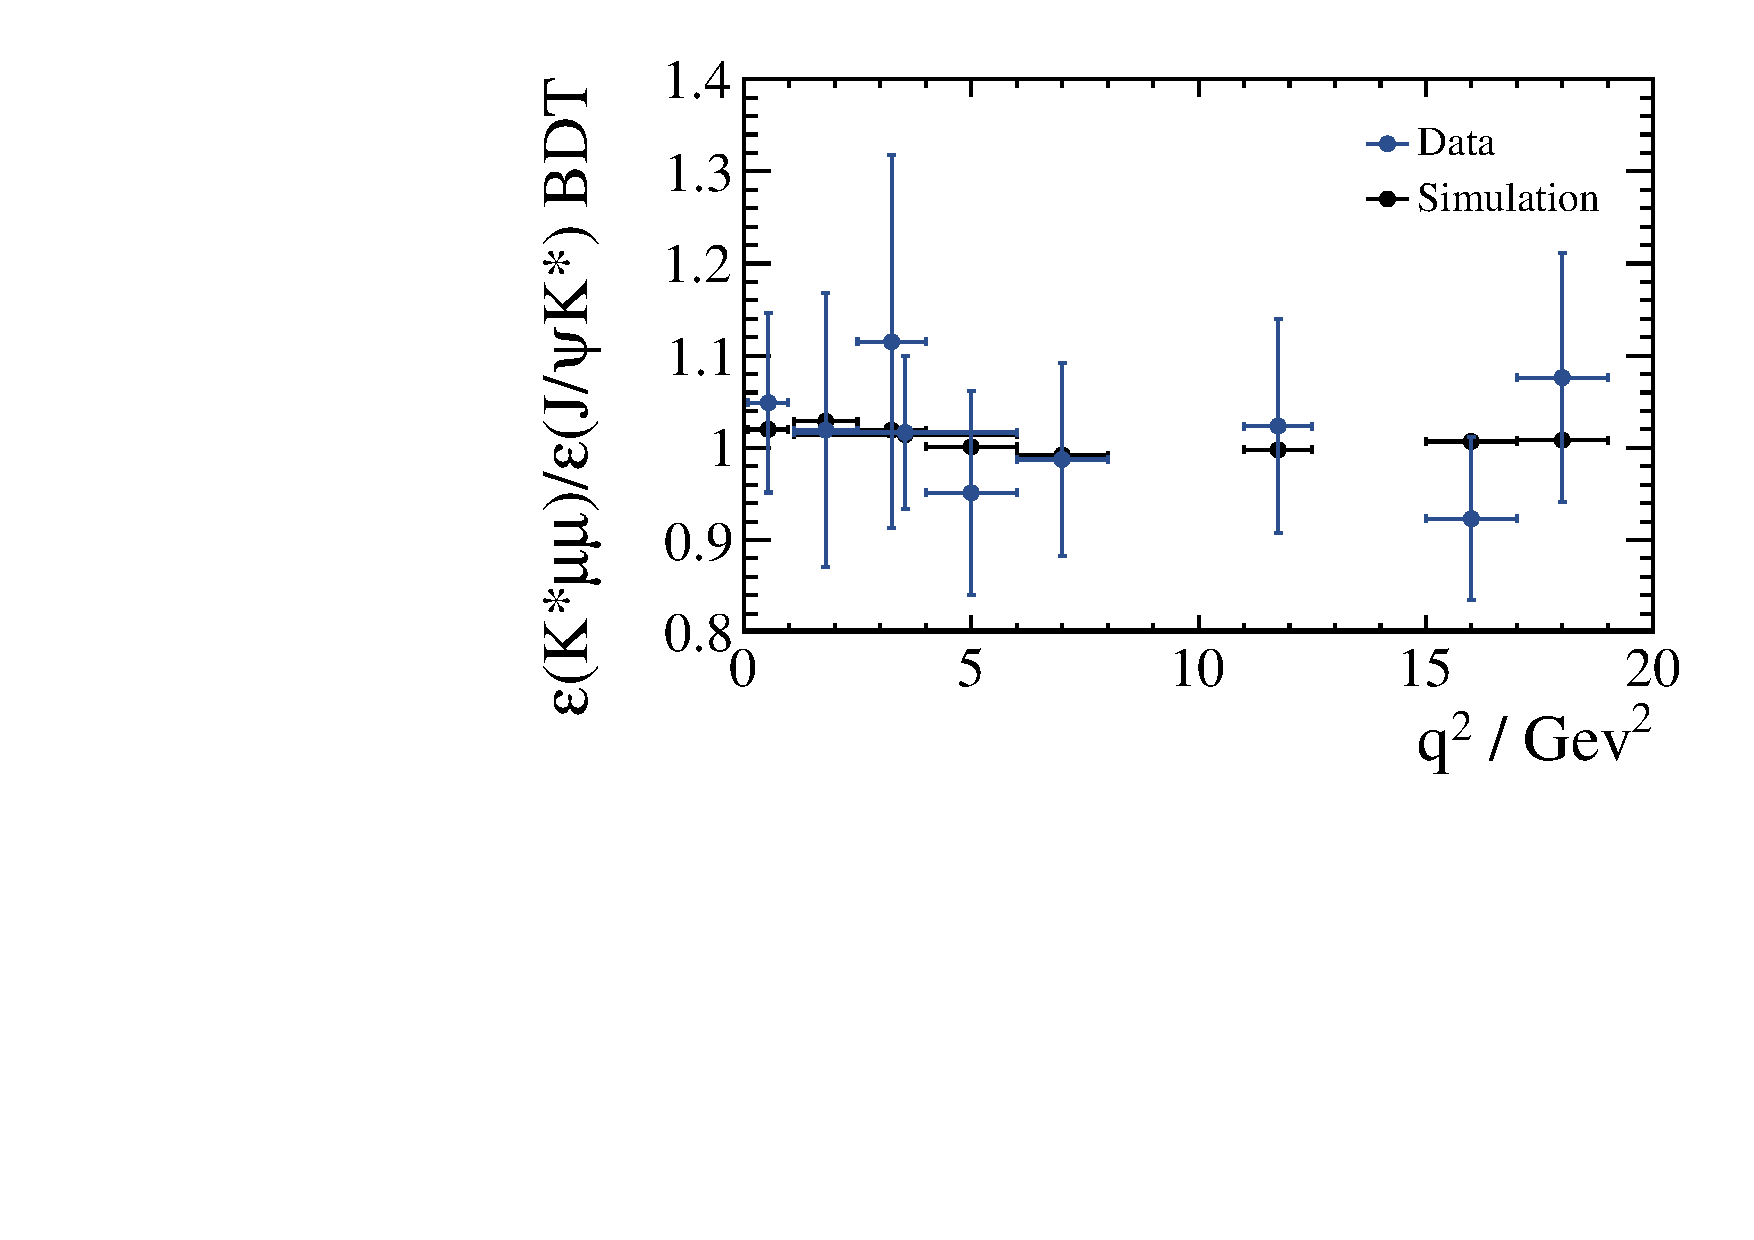
\includegraphics[width=0.48\textwidth]{bdtEffRatio}
    \caption{
      Ratio of the efficiencies of the \bdt selection for a range of \qsq bins, as used in the SM
      \btokstrmumu analysis, with respect to the efficiency for \decay{\Bd}{\jpsi\Kstarz}.
      Data and simulation are shown to be in good agreement.
    }
    \label{fig:bdtEffRatio}
  \end{center}
\end{figure}

At the time of writing, the unblinding procedure is no further than indicated above.
As time progresses the whole dataset will be unblinded.
First in binned distributions
--- which will hide any potential signal, assuming the signal is not extremely obvious ---
in the prompt and displaced regions.
From these distributions toy datasets can be generated and used to convert the local minimum
$p$-value to a global one, the procedure for which is described in \Sect{sec:db:strategy}.
Systematic uncertainties will be evaluated and upper limits will be set for a range of \mass{\db}
and \lifetime{\db}.
If the global $p$-value corresponds to a evidence for a new particle
($3\sigma$ or above) then fits will be used to
determine the best-fit mass and lifetime of the excess.


\subsection[Calculation of $p$-value]
{Calculation of $\boldsymbol{p}$-value}

Firstly, the look-elsewhere effect must be accounted for, which
is done using the method outlined in \Sec{sec:db:pval} using all dimuon pairs from \Bd candidates
that fall within $2.5\stdev$ of the nominal \Bd mass.
Figure~\ref{fig:db:mmumu} shows the unblinded dimuon mass distribution for the prompt and
displaced regions, fitted to fourth order Chebychev polynomials.
A toy dataset is generated using this \PDF, full statistical method is applied to find the
$p$-value at each value of \mass{t}, and thus the minimum $p$-value for a single toy dataset is
extracted.
This process is repeated $10^7$ times, as required to achieve $p$-values corresponding to a
significance of $5\stdev$.
From the minimum $p$-values the fraction of toy datasets with minimum $p$-values less than some
value can be computed, and thus a conversion from local to global minimum $p$-value for any given
toy; and therefore for the data itself.
Figure~\ref{fig:db:mmumu} also shows this cumulative distribution of minimum local $p$-values from
$1.5\e{7}$ datasets along with the asymptotic expectation~\cite{Gross:2010qma}.

\begin{figure}
  \begin{center}
    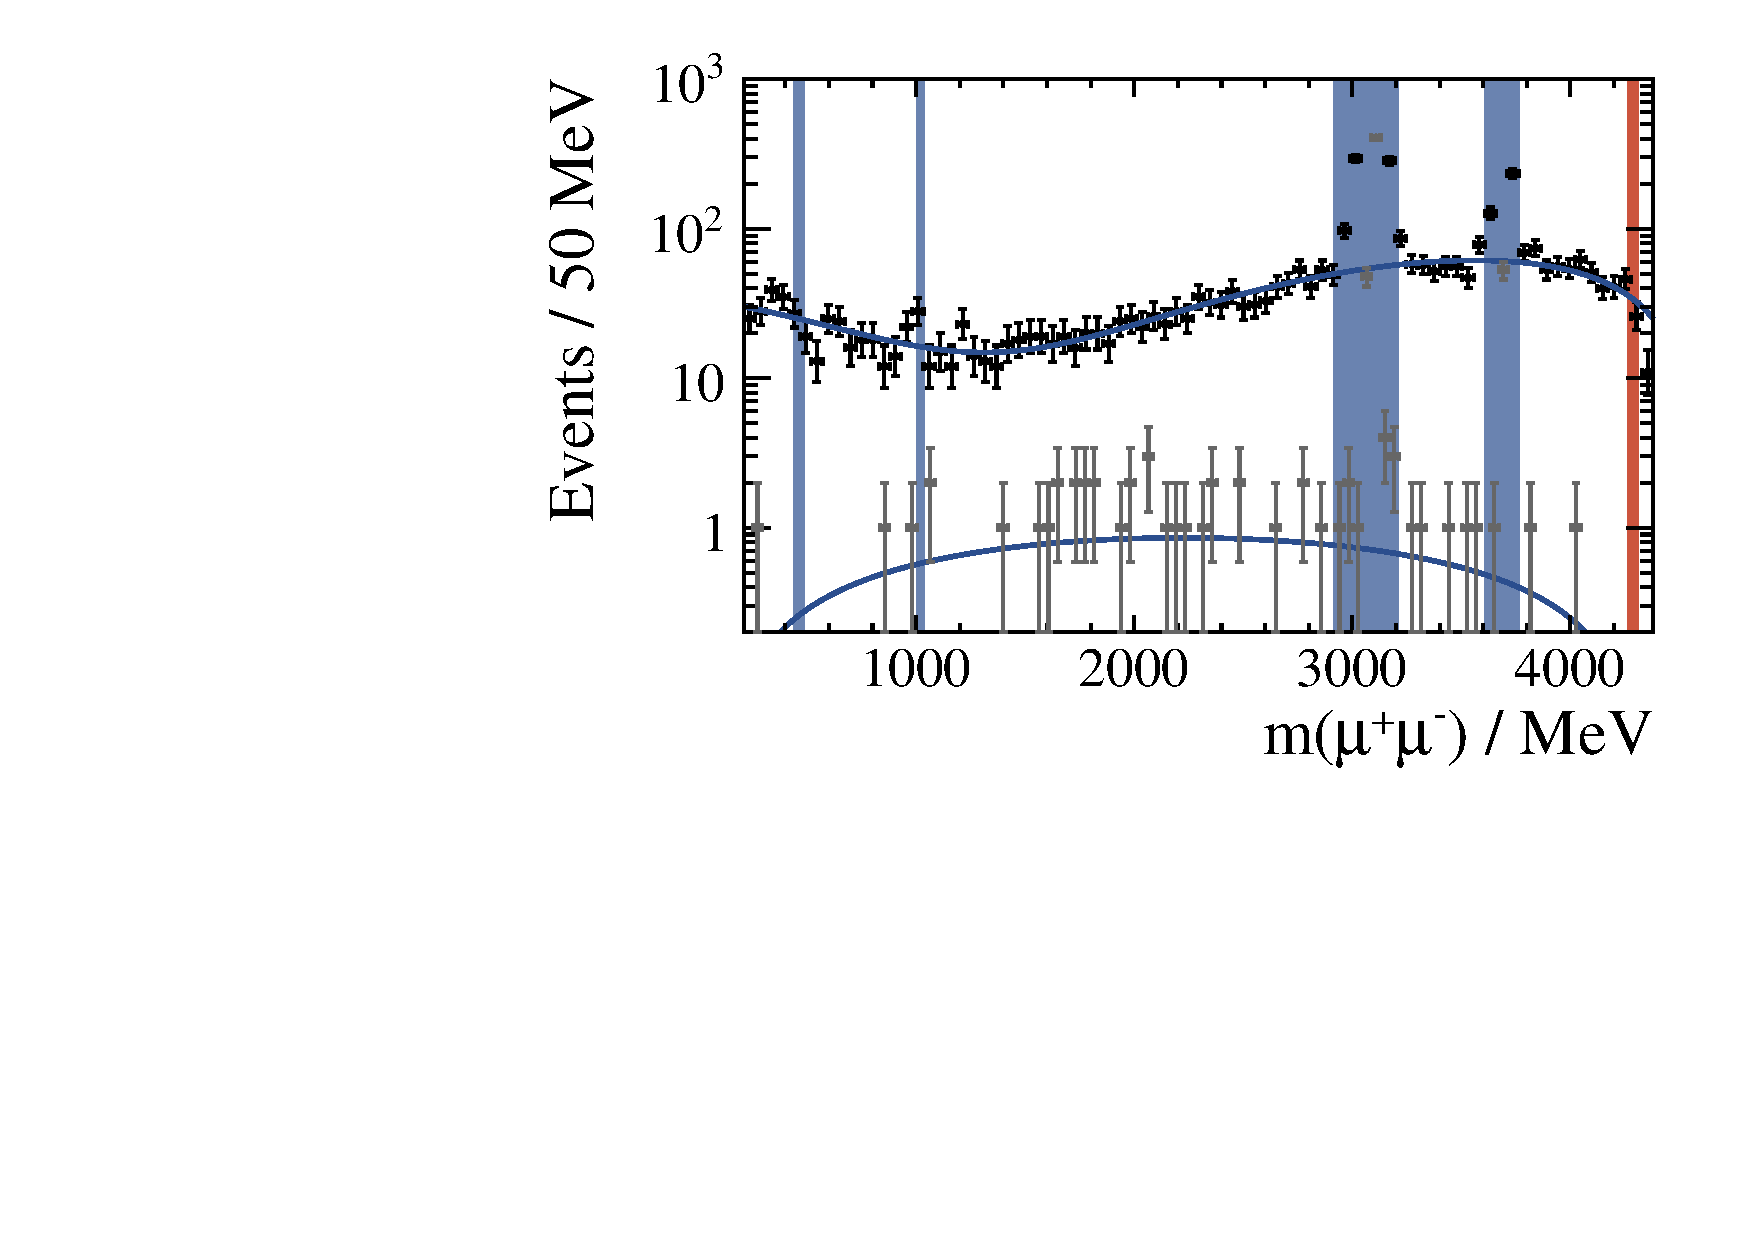
\includegraphics[width=0.48\textwidth]{mxpdf}
    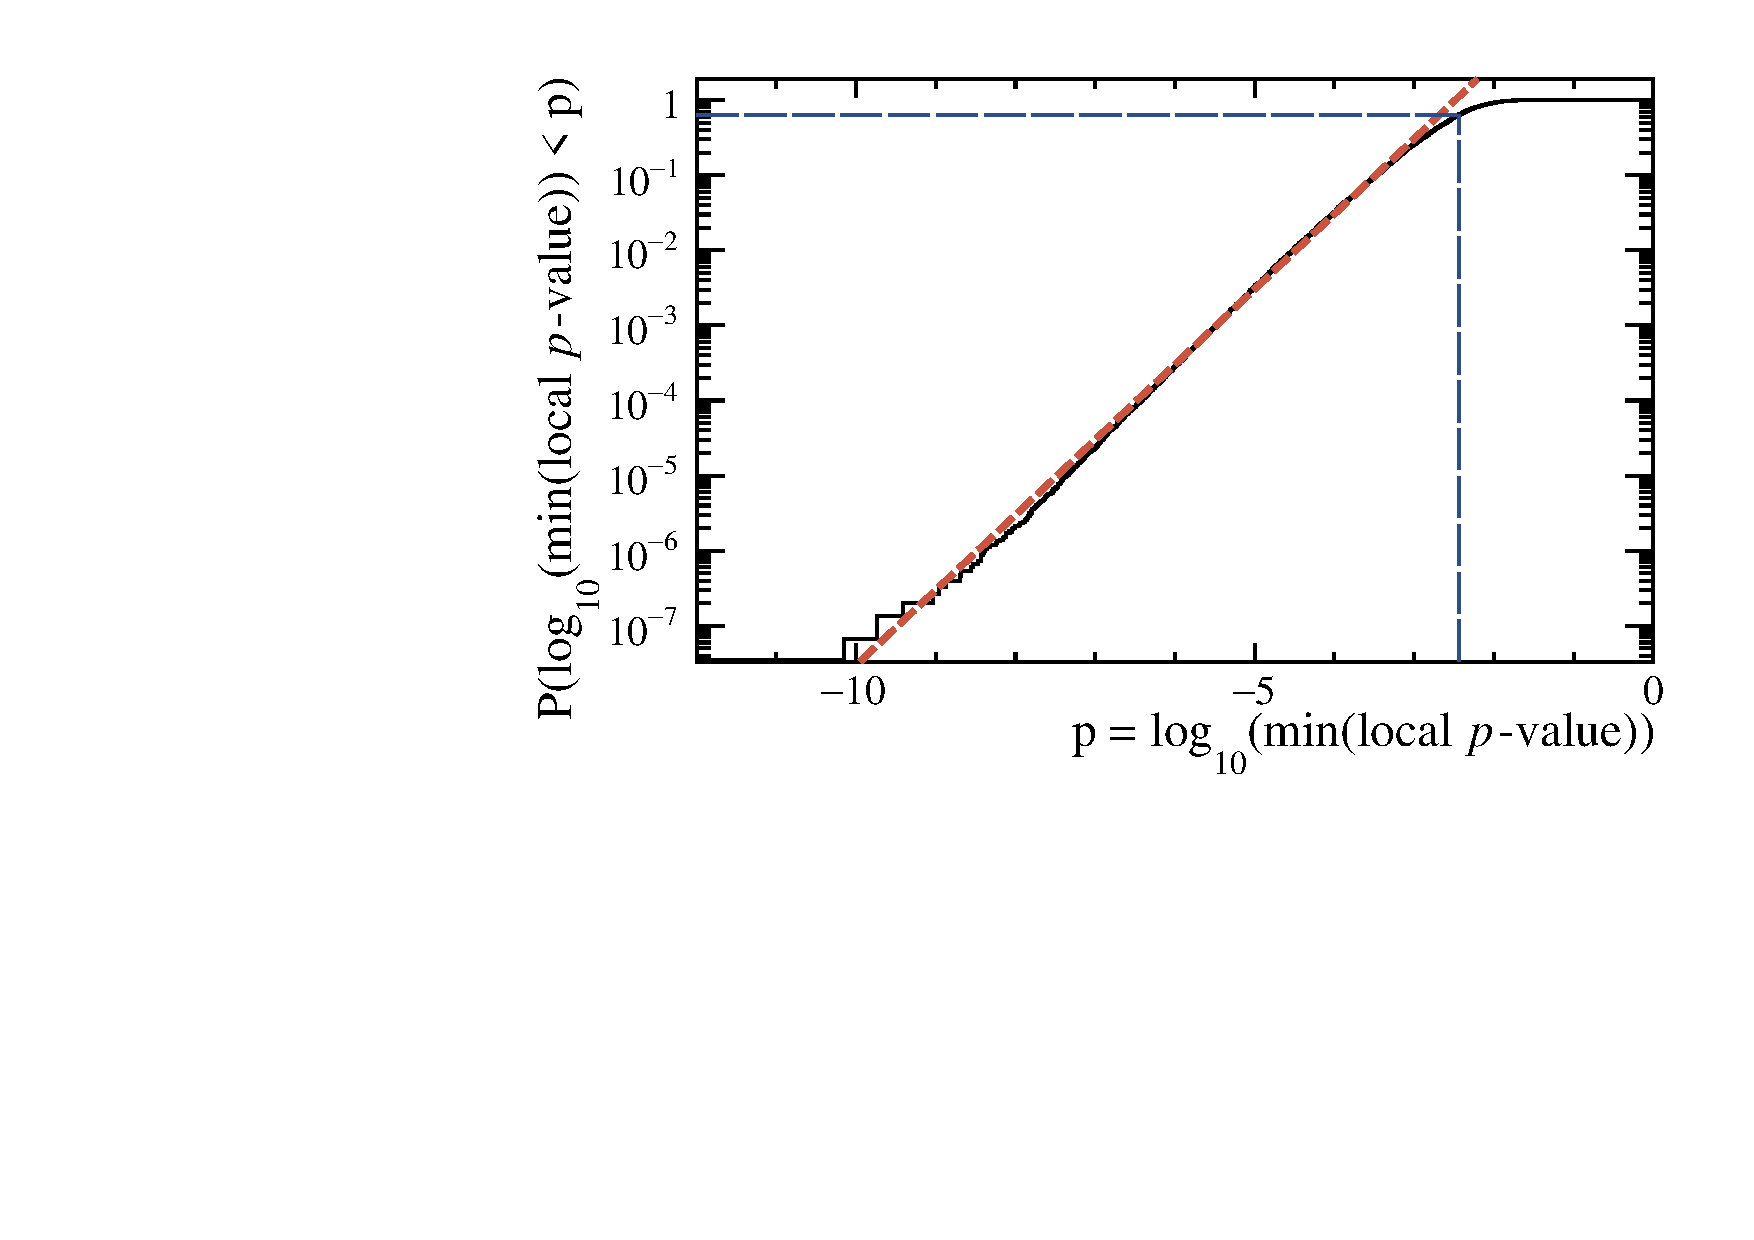
\includegraphics[width=0.48\textwidth]{pvalConversion}
    \caption[]
    {
      FILL IN
    }
    \label{fig:db:mmumu}
  \end{center}
\end{figure}


Scanning values of \mass{t} in the ranges:

The minimum local $p$-value observed in data is $xxx$  at $\mass{\mumu}xxx\mev$,
which corresponds to a global $p$-value of $xxx$; corresponding to a shift in significance of
$xxx\stdev$ to $xxx\stdev$.



%Reference~\cite{Bezrukov:2009yw} considers inflatons with masses in the range
%$1<\mass{\db}<1000\mev$ with lifetimes in the




%From this \PDF ten million toy datasets are generated,
%Ten million are required to be sensitive to

%Using the unblinded
%A fourth order Chebychev polynomial is fit to the unblinded \mass{\mumu} distribution,
%these data
%and
%from this, ten million toy datasets are generated.
%A least ten million are needed in order to be able to probe to $p$-values of $5\stdev$.

%The resulting \qsq distribution is shown in \Fig{fig:res:q2} along with a fit to

%\section{Blinded distributions}
%\label{sec:results}

%Figure~\ref{fig:res:mbvtau}, shows the \db candidate lifetime against \Bd
%mass, it also shows the effect the uBDT cut has on the combinatorial background.
%The lifetime of the \db candidate is also shown as a function of the \db mass, inside and outside
%the \Bd signal region in Fig~\ref{fig:res:mxvtau}.

%%\begin{figure}
  %%\begin{center}
    %%\subfloat[\label{fig:res:mbvtau:all}]{\includegraphics[width=0.48\textwidth]{mb_v_tau}}
    %%\subfloat[\label{fig:res:mbvtau:bdt}]{\includegraphics[width=0.48\textwidth]{mb_v_tau_bdt}}
    %%\caption{\small
      %%Distributions of $\tau(\mumu)$ against $m(\Kstarz\mumu)$ for
      %%candidates from data
      %%\protect\subref{fig:res:mbvtau:all} with no cut, and
      %%\protect\subref{fig:res:mbvtau:bdt} with a cut on the uBDT classifier.
      %%The signal region has been blinded.
    %%}
    %%\label{fig:res:mbvtau}
  %%\end{center}
%%\end{figure}
%%
%%\begin{figure}
  %%\begin{center}
    %%\subfloat[\label{fig:res:mxvtau:all}]{\includegraphics[width=0.48\textwidth]{mx_v_tau}}
    %%\subfloat[\label{fig:res:mxvtau:sig}]{\includegraphics[width=0.48\textwidth]{mx_v_tau_sig}}\\
    %%\subfloat[\label{fig:res:mxvtau:bdtall}]{\includegraphics[width=0.48\textwidth]{mx_v_tau_bdt}}
    %%\subfloat[\label{fig:res:mxvtau:bdtsig}]{\includegraphics[width=0.48\textwidth]{mx_v_tau_sig}}
    %%\caption{\small
      %%Distributions of $\tau(\mumu)$ against $m(\mumu)$ for \db candidates from data in the
      %%\protect\subref{fig:res:mxvtau:all} upper mass sideband, and
      %%\protect\subref{fig:res:mxvtau:sig} signal region (without the uBDT applied).
      %%The Figs.~\protect\subref{fig:res:mxvtau:bdtall} and \protect\subref{fig:res:mxvtau:bdtsig} show the
      %%same, but with uBDT cut applied (blank plots emphasize the analysis is blind).
      %%%\emph{Blank plots will be filled in after unblinding.}
    %%}
    %%\label{fig:res:mxvtau}
  %%\end{center}
%%\end{figure}




%\subsection{Systematic uncertainties}
%Sources of systematic uncertainties that are considered come from the ratio of efficiencies
%ratio of eff
%counting of signal events in prompt and displaced









